% Provenance (never printed): see sources/outline_sources.md (Year 1: gravity and its
% measurement, normal gravity; isostasy, Airy and Pratt; free-air and Bouguer anomalies;
% the geoid). Curves from figdata/bachelor-1/hypsometry.py and gravity_profiles.py;
% exercise and problem values in the Book 3 scratch calculator calc/ch11.py.
\chapter{Isostasie en zwaartekrachtsanomalieën}\label{ch:b1:isostasy-gravity}

In de jaren 1840 stootten landmeters die een meridiaanboog door Noord-India maten op een afwijking die zij niet aan hun instrumenten konden wijten. Tussen twee punten die ongeveer 370 mijl uit elkaar liggen, Kaliana aan de voet van de Himalaya en Kalianpur ver naar het zuiden, overtrof het verschil in \omterm{def:b1:spherical-astronomy:geographic}{breedtegraad} dat door triangulatie werd gevonden het verschil dat uit de sterren werd gevonden met 5.236 boogseconden. De voor de hand liggende schuldige waren de bergen: hun aantrekkingskracht trekt een schietlood naar het noorden, en de astronomen richtten hun instrumenten op het schietlood. In 1855 berekende John Henry Pratt de aantrekking van de Himalaya en van de hoogvlakten daarachter, en vond dat die de afwijking tot 15.885 boogseconden had moeten maken, meer dan drie keer wat werd waargenomen. De bergen trokken veel minder dan hun zichtbare massa vereiste. Datzelfde jaar antwoordde George Airy dat de \omterm{def:b1:layered-earth:layers}{korst} drijft op een dichtere laag, zoals een vlot van stammen op water, zodat hooggelegen land een diepe wortel van lichte steen heeft; Pratt stelde later een ander antwoord voor, steen die lichter is door uitzetting onder de bergen. Beide worden nog steeds onderwezen: de bergen worden onderlaagd door lichte steen die hun massa compenseert. Dit hoofdstuk zet dat idee om in getallen, en laat zien hoe de zwaartekracht, gemeten tot op een miljoenste van haar waarde, de massa's onthult die onder het reliëf verborgen liggen.
% ledger: pratt:himalaya, airy:1855, pratt:1871

\begin{recall}
De wet van Newton voor de gravitatie geeft het veld $g = GM/r^2$ buiten een bolvormige massa $M$; het veld is afgeleid van een gravitatiepotentiaal, en een equipotentiaaloppervlak staat overal loodrecht op het veld (natuurkunde). In een vloeistof in rust neemt de druk met de diepte toe als $\mathrm dp/\mathrm dz = \rho g$, en een drijvend lichaam verplaatst een hoeveelheid vloeistof gelijk aan zijn eigen gewicht (natuurkunde, eerste jaar universiteit). Onder de \omterm{def:b1:layered-earth:lithosphere}{lithosfeer} stroomt de astenosfeer over lange tijden; de \omterm{def:b1:layered-earth:layers}{korst} is lichter dan de \omterm{def:b1:layered-earth:layers}{mantel} eronder (\cref{ch:b1:layered-earth}; Boek 2, klas 11).
\end{recall}

\section{Zwaartekracht en haar meting}

De versnelling van de zwaartekracht aan het oppervlak van de aarde is ongeveer \qty{9.8}{m.s^{-2}}, en de variaties die geologen interesseren zijn een miljoen keer kleiner. Zij worden uitgedrukt in de eenheid van het oude centimeter--gram-stelsel, de gal: $\qty{1}{Gal} = \qty{1}{cm.s^{-2}} = \qty{0.01}{m.s^{-2}}$, zodat
\[
  \qty{1}{\milli\gal} = \qty{e-5}{m.s^{-2}} \approx \num{e-6}\,g .
\]
% ledger: nist:gal
Een veldinstrument meet enkele duizendsten van een milligal; de anomalieën die in dit hoofdstuk worden bestudeerd lopen van een fractie van een milligal boven een begraven ertslichaam tot enkele honderden milligal boven een bergketen.

Zelfs op een kenmerkloze aarde zou de zwaartekracht niet overal gelijk zijn. De aarde draait, zodat wat een schietlood of een zwaartekrachtmeter voelt de som is van de gravitatieaantrekking en het centrifugale effect van de rotatie; en de aarde is afgeplat, zodat de polen dichter bij haar middelpunt liggen dan de evenaar. Beide effecten maken de zwaartekracht aan de evenaar zwakker dan aan de polen. Een geoloog vergelijkt elke meting met een glad \omterm{def:b1:layered-earth:reference-model}{referentiemodel} dat ze alle bevat.

\begin{definition}[Normale zwaartekracht]\label{def:b1:isostasy-gravity:normal-gravity}
\emph{Normale zwaartekracht}\index{normale zwaartekracht} $\gamma$ is de zwaartekracht van een modelaarde: een omwentelingsellipsoïde met de massa en de rotatie van de aarde, zo gekozen dat haar oppervlak een equipotentiaaloppervlak is van haar eigen zwaartekracht (gravitatie plus het centrifugale effect). Op dat oppervlak hangt de normale zwaartekracht alleen van de \omterm{def:b1:spherical-astronomy:geographic}{breedtegraad} af.
\end{definition}

Het ellipsoïde zelf, zijn afplatting en de manier waarop zijn parameters op de werkelijke aarde worden afgestemd, worden bestudeerd in Boek 5. Hier hebben we alleen de zwaartekracht ervan nodig.

\begin{proposition}[De formule voor de normale zwaartekracht]\label{prop:b1:isostasy-gravity:normal-formula}
Op het referentie-ellipsoïde dat in 1980 werd aangenomen, is de \omterm{def:b1:isostasy-gravity:normal-gravity}{normale zwaartekracht} op de geografische \omterm{def:b1:spherical-astronomy:geographic}{breedtegraad} $\varphi$, in haar gebruikelijke reeksvorm,
\[
  \gamma(\varphi) = \qty{9.780327}{m.s^{-2}}\,\bigl(1 + 0.0053024\sin^2\varphi
  - 0.0000058\sin^2 2\varphi\bigr).
\]
\end{proposition}
\admitted
% ledger: moritz:grs80

Dat geeft \qty{9.780327}{m.s^{-2}} aan de evenaar, \qty{9.806200}{m.s^{-2}} bij \ang{45} en \qty{9.832186}{m.s^{-2}} aan de polen: een verschil van \qty{5186}{\milli\gal} van evenaar tot pool. De rotatie alleen verklaart het grootste deel ervan. Met de siderische dag van \qty{23.9345}{h} is de hoeksnelheid $\omega = 2\pi/\qty{86164}{s} = \qty{7.292e-5}{rad.s^{-1}}$, en de centrifugale versnelling aan de evenaar, $\omega^2 a$ met $a = \qty{6378.137}{km}$, bedraagt \qty{0.0339}{m.s^{-2}}, of \qty{3392}{\milli\gal}; de afplatting levert de rest (\cref{exo:b1:isostasy-gravity:2}).
% ledger: earth:Trot, earth:Req, earth:geq, earth:gpole

Zwaartekracht wordt op twee manieren gemeten. Een \emph{absolute} zwaartekrachtmeter laat een testmassa in een vacuümkamer vallen en volgt haar vrije val met een laserinterferometer, gemeten met een atoomklok: de versnelling volgt rechtstreeks uit afstand en tijd. Een \emph{relatieve} zwaartekrachtmeter is een massa aan een veer, waarvan de uitrekking met de zwaartekracht verandert; hij is licht en snel, maar geeft alleen verschillen tussen plaatsen, en hij drijft af, zodat een meetcampagne terugkeert naar een basisstation waarvan de zwaartekracht bekend is. De beste absolute instrumenten zijn nauwkeurig tot ongeveer een microgal, een deel per miljard van $g$.
% ledger: ngs:absolute-gravity

\begin{inthefield}[Een zwaartekrachtcampagne op land]
\begin{minipage}[t]{0.55\linewidth}\vspace{0pt}
Een zwaartekrachtcampagne is een langzame tocht van station naar station. Bij elk station zet de geofysicus de relatieve zwaartekrachtmeter op zijn statief, waterpast hem, wacht tot de veer tot rust komt en neemt enkele aflezingen; een ontvanger voor satellietpositionering ernaast legt de positie en de hoogte van het station vast. Elke paar uur gaat het team terug naar het basisstation, zodat de drift van de veer kan worden gemeten en verwijderd. De hoogte telt even zwaar als de zwaartekracht: zoals de volgende paragraaf laat zien, neemt de zwaartekracht met \qty{0.3086}{\milli\gal} af voor elke meter hoogte, dus een hoogte die \qty{1}{cm} verkeerd is, bederft de aflezing met \qty{3}{\micro\gal}. % ledger: usgs73:reduction
\end{minipage}\hfill
\begin{minipage}[t]{0.42\linewidth}\vspace{0pt}
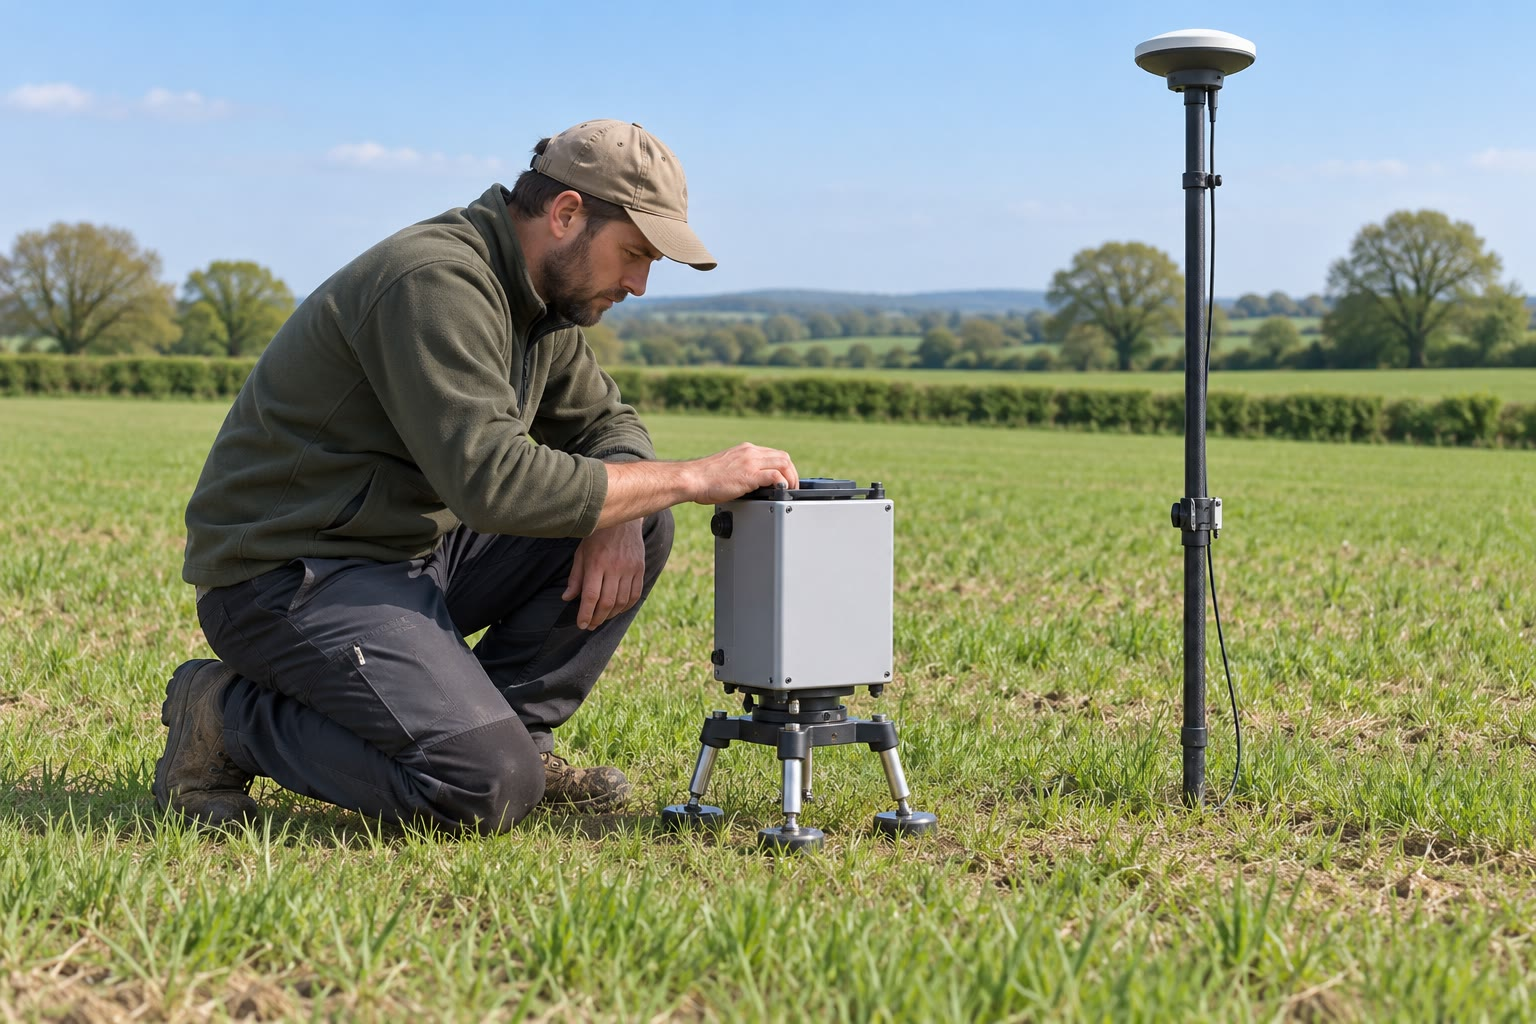
\includegraphics[width=\linewidth]{images/book3/ai/b1-gravity-survey.jpg}

{\scriptsize Een veldzwaartekrachtmeter op zijn statief, met een antenne voor satellietpositionering ernaast (door AI gegenereerde illustratie).}
\end{minipage}
\end{inthefield}

\section{Isostasie}

De compensatie die Airy en Pratt voor de Himalaya bedachten, is een geval van een algemene toestand van de buitenste lagen van de aarde.

\begin{definition}[Isostasie; compensatiediepte]\label{def:b1:isostasy-gravity:isostasy}
Een gebied is in \emph{isostasie}\index{isostasie}, of isostatisch evenwicht, wanneer er een diepte bestaat, de \emph{compensatiediepte}\index{compensatiediepte}, waarop de druk op elk punt van het horizontale oppervlak dezelfde is, wat het reliëf erboven ook is. Onder de compensatiediepte gedragen de gesteenten zich als een vloeistof in rust; erboven drijven de kolommen van \omterm{def:b1:layered-earth:layers}{korst} en \omterm{def:b1:layered-earth:layers}{mantel} erop.
\end{definition}

\begin{proposition}[Gelijke massa's boven de compensatiediepte]\label{prop:b1:isostasy-gravity:equal-mass}
Als de zwaartekracht $g$ langs alle kolommen dezelfde is, is een gebied in \omterm{def:b1:isostasy-gravity:isostasy}{isostasie} met \omterm{def:b1:isostasy-gravity:isostasy}{compensatiediepte} $z_c$ dan en slechts dan wanneer elke verticale kolom van eenheidsdoorsnede, van het oppervlak tot $z_c$, dezelfde massa bevat.
\end{proposition}

\begin{proof}
In elke kolom zijn de gesteenten in hydrostatisch evenwicht, zodat
$\mathrm dp/\mathrm dz = \rho(z)\,g$, met de diepte $z$ naar beneden geteld. De druk aan het oppervlak is atmosferisch, overal dezelfde (en verwaarloosbaar).
Integrerend vanaf het oppervlak $z_s$ van de kolom tot $z_c$ volgt
\[
  p(z_c) = p_0 + g\int_{z_s}^{z_c}\rho(z)\,\mathrm dz ,
\]
waarbij de integraal de massa van de kolom per oppervlakte-eenheid is. De drukken op
$z_c$ zijn dan en slechts dan gelijk wanneer deze massa's gelijk zijn.
\end{proof}

Twee eenvoudige manieren om de massa's te verdelen geven de twee klassieke modellen (figuur hieronder).

\begin{proposition}[Airy-isostasie]\label{prop:b1:isostasy-gravity:airy}
Laat de \omterm{def:b1:layered-earth:layers}{korst} een uniforme dichtheid $\rho_c$ hebben en een dikte $H$ waar haar oppervlak op zeeniveau ligt, boven een \omterm{def:b1:layered-earth:layers}{mantel} met dichtheid $\rho_m > \rho_c$. In isostatisch evenwicht geldt:
\begin{enumerate}
  \item waar het oppervlak zich op een hoogte $h$ boven zeeniveau bevindt, heeft de \omterm{def:b1:layered-earth:layers}{korst} een wortel van diepte $r = h\,\rho_c/(\rho_m - \rho_c)$ onder de normale \omterm{def:b1:layered-earth:layers}{korst}, en een dikte $H + h + r$;
  \item waar het oppervlak zich op een diepte $d$ onder zeeniveau bevindt, onder water met dichtheid $\rho_w$, heeft de \omterm{def:b1:layered-earth:layers}{korst} een antiwortel: haar basis is opgetild met $r' = d\,(\rho_c - \rho_w)/(\rho_m - \rho_c)$, en haar dikte is $H - d - r'$.
\end{enumerate}
Dit is \emph{Airy-isostasie}\index{Airy-isostasie}: compensatie door veranderingen van dikte bij constante dichtheid.
\end{proposition}

\begin{proof}
Neem de \omterm{def:b1:isostasy-gravity:isostasy}{compensatiediepte} net onder de diepste wortel en vergelijk elke kolom met de normale. (1) De hoge kolom heeft \omterm{def:b1:layered-earth:layers}{korst} in plaats van \omterm{def:b1:layered-earth:layers}{mantel} over de diepte $r$, en \omterm{def:b1:layered-earth:layers}{korst} over de hoogte $h$ waar de normale kolom niets heeft: gelijke massa's vereisen $\rho_c(h + r) = \rho_m r$, dat wil zeggen
$r(\rho_m - \rho_c) = \rho_c h$. (2) De lage kolom heeft water in plaats van \omterm{def:b1:layered-earth:layers}{korst} over de diepte $d$, en \omterm{def:b1:layered-earth:layers}{mantel} in plaats van \omterm{def:b1:layered-earth:layers}{korst} over $r'$: gelijke massa's vereisen $\rho_w d + \rho_m r' = \rho_c(d + r')$, dat wil zeggen $r'(\rho_m - \rho_c) =
d(\rho_c - \rho_w)$.
\end{proof}

\begin{proposition}[Pratt-isostasie]\label{prop:b1:isostasy-gravity:pratt}
Laat elke kolom eindigen op dezelfde \omterm{def:b1:isostasy-gravity:isostasy}{compensatiediepte} $D$ onder zeeniveau, met een uniforme dichtheid in elke kolom, $\rho_0$ waar het oppervlak op zeeniveau ligt. In isostatisch evenwicht heeft een kolom waarvan het oppervlak op een hoogte $h$ staat de dichtheid
\[
  \rho(h) = \rho_0\,\frac{D}{D + h},
\]
en een kolom onder een waterdiepte $d$ heeft de dichtheid $\rho = (\rho_0 D - \rho_w d)/(D - d)$. Dit is \emph{Pratt-isostasie}\index{Pratt-isostasie}: compensatie door veranderingen van dichtheid bij constante diepte.
\end{proposition}

\begin{proof}
Gelijke massa's boven $D$: $\rho(h)(D + h) = \rho_0 D$ voor de hoge kolom, en
$\rho_w d + \rho(D - d) = \rho_0 D$ voor de lage.
\end{proof}

Met $\rho_c = \qty{2700}{kg.m^{-3}}$ en $\rho_m = \qty{3300}{kg.m^{-3}}$ is de wortel van Airy $h\times2700/600 = 4.5\,h$: een gebergte van \qty{2}{km} hoog heeft een wortel van \qty{9}{km}, een plateau van \qty{4}{km} hoog een van \qty{18}{km}. In het model van Pratt met $D = \qty{100}{km}$ en $\rho_0 = \qty{2700}{kg.m^{-3}}$ hebben dezelfde twee kolommen de dichtheden 2647 en \qty{2596}{kg.m^{-3}}, respectievelijk twee en vier procent lichter. Beide modellen balanceren dezelfde massa's; zij verschillen in waar de lichte steen zit, en dat kan de seismologie zien: Airy voorspelt een \omterm{def:b1:layered-earth:discontinuity}{Moho} die onder de bergen dieper wordt, Pratt een vlakke.

\begin{omfigure}
\begin{tikzpicture}[x=0.55cm, y=0.05cm, font=\scriptsize]
% columns computed in calc/ch11.py: Airy roots 9 and 18 km, Pratt densities 2647 and 2596 kg/m3;
% heights above sea level drawn five times larger than depths
\begin{scope}
  \node[font=\small] at (4.5,30) {(a) model van Airy};
  \fill[omLithGranite!45] (0,0) rectangle (3,-35);
  \fill[omLithGranite!45] (3,10) rectangle (6,-44);
  \fill[omLithGranite!45] (6,20) rectangle (9,-53);
  \fill[omLithPeridotite!45] (0,-35) rectangle (3,-60);
  \fill[omLithPeridotite!45] (3,-44) rectangle (6,-60);
  \fill[omLithPeridotite!45] (6,-53) rectangle (9,-60);
  \draw (0,-60) -- (0,0) -- (3,0) -- (3,10) -- (6,10) -- (6,20) -- (9,20) -- (9,-60);
  \draw (3,0) -- (3,-60) (6,10) -- (6,-60);
  \draw[thick] (0,-35) -- (3,-35) -- (3,-44) -- (6,-44) -- (6,-53) -- (9,-53);
  \draw[densely dashed] (-0.3,-60) -- (9.3,-60);
  \draw[black!50, densely dotted] (-0.3,0) -- (0,0);
  \node[anchor=east] at (-0.3,0) {zeeniveau};
  \node[anchor=east] at (-0.3,-35) {35};
  \node[anchor=east] at (-0.3,-60) {60 km};
  \node at (1.5,-17) {2700}; \node at (4.5,-20) {2700}; \node at (7.5,-24) {2700};
  \node at (1.5,-50) {3300};
  \node[anchor=south] at (1.5,0) {$h = 0$};
  \node[anchor=south] at (4.5,10) {$h = 2$};
  \node[anchor=south] at (7.5,20) {$h = 4$};
  \draw[black!45, densely dotted] (3,-35) -- (9,-35);
  \node at (4.5,-39.5) {wortel 9};
  \node at (7.5,-44) {wortel 18};
\end{scope}
\begin{scope}[xshift=7.9cm]
  \node[font=\small] at (4.5,30) {(b) model van Pratt};
  \fill[omLithGranite!45] (0,0) rectangle (3,-100);
  \fill[omLithGranite!36] (3,10) rectangle (6,-100);
  \fill[omLithGranite!27] (6,20) rectangle (9,-100);
  \draw (0,-100) -- (0,0) -- (3,0) -- (3,10) -- (6,10) -- (6,20) -- (9,20) -- (9,-100);
  \draw (3,0) -- (3,-100) (6,10) -- (6,-100);
  \draw[densely dashed] (-0.3,-100) -- (9.3,-100);
  \draw[black!50, densely dotted] (-0.3,0) -- (0,0);
  \node[anchor=east] at (-0.3,0) {zeeniveau};
  \node[anchor=east] at (-0.3,-100) {$D = 100$ km};
  \node at (1.5,-50) {2700}; \node at (4.5,-50) {2647}; \node at (7.5,-50) {2596};
  \node[anchor=south] at (1.5,0) {$h = 0$};
  \node[anchor=south] at (4.5,10) {$h = 2$};
  \node[anchor=south] at (7.5,20) {$h = 4$};
\end{scope}
\end{tikzpicture}

\par\smallskip{\small De twee klassieke modellen van \omterm{def:b1:isostasy-gravity:isostasy}{isostasie}, voor drie kolommen die 0, 2 en \qty{4}{km} boven zeeniveau staan (hoogten vijfmaal overdreven ten opzichte van de diepten; dichtheden in \unit{kg.m^{-3}}). (a) Airy: één korstdichtheid, een wortel die 4.5 keer de hoogte is. (b) Pratt: één \omterm{def:b1:isostasy-gravity:isostasy}{compensatiediepte}, lichtere kolommen onder hoger land. Elke kolom draagt dezelfde massa per oppervlakte-eenheid boven de gestreepte \omterm{def:b1:isostasy-gravity:isostasy}{compensatiediepte}.}
\label{fig:b1:isostasy-gravity:models}
\end{omfigure}

\omterm{def:b1:isostasy-gravity:isostasy}{Isostasie} is een uitspraak over brede gebieden op lange tijdschalen. De astenosfeer geeft alleen mee aan belastingen die duizenden jaren aanhouden, en de \omterm{def:b1:layered-earth:lithosphere}{lithosfeer} erboven is stijf genoeg om een smalle belasting door buiging over een breed gebied te spreiden, zoals een plank een gewicht draagt: een enkele vulkaan hoeft niet onder zichzelf te worden gecompenseerd; deze buiging van de \omterm{def:b1:layered-earth:lithosphere}{lithosfeer} wordt bestudeerd in Boek 5. Onder grote bergketens is de \omterm{def:b1:layered-earth:layers}{korst} veel dikker dan haar continentale gemiddelde van ongeveer \qty{30}{km}: het beeld van Airy, wortels van lichte \omterm{def:b1:layered-earth:layers}{korst}, is voor bergketens het nauwste. Dat van Pratt, lichtere steen op constante diepte, verklaart de middenoceanische ruggen, die hoog staan boven een bovenmantel die lichter is door haar hogere temperatuur.
% ledger: usgs:crust-thickness

\subsection*{De twee niveaus van de aarde}

\omterm{def:b1:isostasy-gravity:isostasy}{Isostasie} organiseert het reliëf van de hele planeet. Die verdeling wordt samengevat door één kromme.

\begin{definition}[Hypsometrische kromme]\label{def:b1:isostasy-gravity:hypsometry}
De \emph{hypsometrische kromme}\index{hypsometrische kromme} van een planeet geeft voor elke fractie $f$ van haar oppervlak de hoogte $z(f)$ die precies door die fractie wordt overschreden. Zij is de cumulatieve verdeling van de hoogte, van boven af gelezen.
\end{definition}

Om haar uit een rasterhoogtemodel te tekenen, moet elke rastercel met haar oppervlakte worden gewogen. Op een raster van één graad in breedte- en \omterm{def:b1:spherical-astronomy:geographic}{lengtegraad} heeft de cel tussen de breedtegraden $\varphi_1$ en $\varphi_2$ de oppervlakte $R^2\,\Delta\lambda\,(\sin\varphi_2 - \sin\varphi_1)$, die naar de polen toe krimpt; opgeteld over alle cellen geven de oppervlakten precies $4\pi R^2$. De cellen naar hoogte sorteren en hun oppervlakten opstapelen geeft de kromme van de figuur hieronder. Zij toont dat \qty{70.9}{\percent} van het oppervlak onder zeeniveau ligt; dat de gemiddelde hoogte van het land ongeveer \qty{0.8}{km} is en de gemiddelde diepte van de oceaan ongeveer \qty{3.7}{km}; en dat het meeste oppervlak tot één van twee vlakke trappen behoort, de continentale platformen vlak bij zeeniveau en de abyssale vloer tussen ongeveer 3.5 en \qty{6}{km} diep, verbonden door een steile val.
% computed in figdata/bachelor-1/hypsometry.py (fraction 0.709, land 793 m, ocean 3692 m); ledger: data:etopo1, wss:ocean-cover

Een planeet met één soort \omterm{def:b1:layered-earth:layers}{korst}, waarvan het reliëf willekeurig is opgeheven en afgesleten, zou één niveau hebben, met hoogten die eromheen verspreid liggen. De aarde heeft er twee, omdat zij twee soorten \omterm{def:b1:layered-earth:layers}{korst} heeft in isostatisch evenwicht: de dikke, lichte continentale \omterm{def:b1:layered-earth:layers}{korst} drijft hoog, de dunne, dichte oceanische \omterm{def:b1:layered-earth:layers}{korst} laag (Boek 2, klas 11). \Cref{exo:b1:isostasy-gravity:8} laat zien dat het model van Airy met één korstdichtheid beide niveaus niet kan voortbrengen met de waargenomen korstdiktes.

\begin{omfigure}
\begin{tikzpicture}
\begin{axis}[omrecord, width=0.84\linewidth, height=6.4cm, xmin=0, xmax=100, ymin=-11, ymax=9,
  xlabel={fractie van het oppervlak van de aarde dat hoger ligt (\unit{\percent})},
  ylabel={hoogte (km)}, xtick={0,10,...,100}, ytick={-10,-8,...,8},
  tick label style={font=\scriptsize}, label style={font=\small}, clip=true]
% computed in figdata/bachelor-1/hypsometry.py; ledger: data:etopo1
\addplot[name path=hyps, very thick, black] table[x=area_pc, y expr=\thisrow{elev}/1000] {figdata/out/bachelor-1-hypsometry-curve.dat};
\path[name path=sea] (axis cs:0,0) -- (axis cs:100,0);
\addplot[omSea!60] fill between[of=hyps and sea, soft clip={domain=29.1:100}];
\addplot[omHypsLandC!80] fill between[of=hyps and sea, soft clip={domain=0:29.1}];
\draw[black!60, densely dotted] (axis cs:0,0) -- (axis cs:100,0);
\draw[black!60, densely dashed] (axis cs:29.1,-11) -- (axis cs:29.1,9);
\draw[omSea!60!black, densely dashed] (axis cs:29.1,-3.692) -- (axis cs:100,-3.692);
\draw[omHypsLandF, densely dashed] (axis cs:0,0.793) -- (axis cs:29.1,0.793);
\node[font=\scriptsize, anchor=south east] at (axis cs:99,0.1) {zeeniveau};
\node[font=\scriptsize, anchor=south, align=center] at (axis cs:18,1.0) {gemiddelde\\landhoogte \qty{0.79}{km}};
\node[font=\scriptsize, anchor=north west, align=left] at (axis cs:31,-3.9) {gemiddelde\\oceaandiepte \qty{3.69}{km}};
\node[font=\scriptsize, anchor=north west, align=left] at (axis cs:30.5,6.5) {land: \qty{29.1}{\percent}\\van het oppervlak};
\node[font=\scriptsize, anchor=north, align=center] at (axis cs:17,-0.5) {continentaal\\platform};
\node[font=\scriptsize] at (axis cs:62,-5.2) {abyssale vloer};
\end{axis}
\end{tikzpicture}

\par\smallskip{\small De \omterm{def:b1:isostasy-gravity:hypsometry}{hypsometrische kromme} van de aarde, uit het wereldwijde reliëfmodel ETOPO1 op één graad, elke cel gewogen naar haar oppervlakte (boven Antarctica en Groenland de top van het ijs). De twee bijna vlakke delen van de kromme zijn de continentale platformen vlak bij zeeniveau en de diepe oceaanbodem.}
\label{fig:b1:isostasy-gravity:hypsometry}
\end{omfigure}

\section{Zwaartekrachtsanomalieën}

\subsection*{Twee correcties}

Een zwaartekrachtmeter op een heuvel staat verder van het middelpunt van de aarde dan een op zeeniveau, en staat op een laag gesteente die de andere niet heeft. Beide effecten worden berekend voordat de meting met de \omterm{def:b1:isostasy-gravity:normal-gravity}{normale zwaartekracht} wordt vergeleken.

\begin{proposition}[Vrije-luchtgradiënt]\label{prop:b1:isostasy-gravity:free-air}
Buiten een bolvormige aarde met straal $R$ neemt de zwaartekracht met de hoogte $h$ af met de snelheid
\[
  \frac{\mathrm dg}{\mathrm dh} = -\frac{2g}{R}\,;
\]
aan het oppervlak is $2g/R \approx \qty{3.08e-6}{s^{-2}}$, ongeveer \qty{0.308}{\milli\gal} per meter.
\end{proposition}

\begin{proof}
$g(r) = GM/r^2$, dus $\mathrm dg/\mathrm dr = -2GM/r^3 = -2g(r)/r$; bij $r = R$,
met $g = \qty{9.820}{m.s^{-2}}$ en $R = \qty{6371}{km}$, is $2g/R =
\qty{3.083e-6}{s^{-2}}$.
\end{proof}
% ledger: earth:gmean, earth:Rmean

De afplatting en de rotatie veranderen de gradiënt een beetje; de in de praktijk gebruikte waarde is \qty{0.3086}{\milli\gal.m^{-1}}.
% ledger: usgs73:reduction

\begin{proposition}[Bouguer-plaat]\label{prop:b1:isostasy-gravity:slab}
Een oneindige horizontale plaat met dikte $h$ en uniforme dichtheid $\rho$ trekt een punt erbuiten aan met de verticale versnelling
\[
  g_B = 2\pi G\rho h ,
\]
ongeacht de afstand van het punt tot de plaat. Numeriek is $2\pi G =
\qty{0.0419}{\milli\gal}$ per meter dikte per \qty{1000}{kg.m^{-3}} dichtheid.
\end{proposition}

\begin{proof}
Plaats het punt in de oorsprong en snijd de plaat in dunne ringen die coaxiaal zijn met de verticale erdoorheen. Een ring op de afstand $z$ onder het punt, met straal $s$, breedte $\mathrm ds$ en dikte $\mathrm dz$, heeft de massa $\rho\,2\pi s\,\mathrm ds\,\mathrm dz$, allemaal op de afstand $\sqrt{s^2 + z^2}$; door symmetrie is haar aantrekking verticaal, gelijk aan de aantrekking van elk element maal de cosinus $z/\sqrt{s^2+z^2}$ van zijn hoek met de verticale:
\[
  \mathrm dg = G\,\frac{\rho\,2\pi s\,\mathrm ds\,\mathrm dz}{s^2 + z^2}\,
  \frac{z}{\sqrt{s^2 + z^2}} .
\]
Voor één laag geldt $\int_0^\infty s\,(s^2 + z^2)^{-3/2}\,\mathrm ds =
\bigl[-(s^2 + z^2)^{-1/2}\bigr]_0^\infty = 1/z$, dus trekt de laag aan met
$2\pi G\rho\,\mathrm dz$, onafhankelijk van $z$. Het optellen van de lagen over de dikte $h$ geeft $2\pi G\rho h$. Met $G = \qty{6.674e-11}{m^3.kg^{-1}.s^{-2}}$,
$2\pi G\times\qty{1000}{kg.m^{-3}}\times\qty{1}{m} = \qty{4.19e-7}{m.s^{-2}} =
\qty{0.0419}{\milli\gal}$.
\end{proof}
% ledger: const:G

\begin{definition}[Zwaartekrachtsanomalieën]\label{def:b1:isostasy-gravity:anomalies}
Laat $g$ de zwaartekracht zijn die is gemeten op een station met \omterm{def:b1:spherical-astronomy:geographic}{breedtegraad} $\varphi$ en hoogte $h$ boven zeeniveau.
\begin{itemize}
  \item Een \emph{zwaartekrachtsanomalie}\index{zwaartekrachtsanomalie} is het verschil tussen de gemeten zwaartekracht, gecorrigeerd naar een gemeenschappelijk niveau, en de \omterm{def:b1:isostasy-gravity:normal-gravity}{normale zwaartekracht} op dezelfde \omterm{def:b1:spherical-astronomy:geographic}{breedtegraad}.
  \item De \emph{vrije-luchtcorrectie}\index{vrije-luchtcorrectie} is
        $+\qty{0.3086}{\milli\gal.m^{-1}}\times h$: zij voegt de afname van de zwaartekracht met de hoogte weer toe. De \emph{vrije-luchtanomalie}\index{vrije-luchtanomalie} is
        $\Delta g_{\mathrm{FA}} = g + 0.3086\,h - \gamma(\varphi)$.
  \item De \emph{Bouguer-correctie}\index{Bouguer-correctie} is $-2\pi G\rho h$:
        zij verwijdert de aantrekking van het gesteente tussen het station en zeeniveau, behandeld als een plaat met dichtheid $\rho$, conventioneel \qty{2670}{kg.m^{-3}}, wat \qty{0.112}{\milli\gal} per meter geeft. De \emph{Bouguer-anomalie}\index{Bouguer-anomalie} is $\Delta g_{\mathrm B} = \Delta g_{\mathrm{FA}} - 2\pi G\rho h$.
\end{itemize}
\end{definition}
% ledger: usgs73:reduction, swisstopo:bouguer-map

De plaat is een grof model van de grond rond een station in ruw terrein: dalen onder het station worden geteld als gesteente dat er niet is, heuvels erboven trekken omhoog en tellen helemaal niet mee. Een derde reductie, de reliëfcorrectie, berekend uit een \omterm{def:b1:geological-maps:dem}{digitaal hoogtemodel}, verwijdert beide fouten. Op zee verdwijnt de \omterm{def:b1:isostasy-gravity:anomalies}{vrije-luchtcorrectie}, en de Bouguer-reductie vervangt het water door gesteente.

\begin{method}[Een zwaartekrachtsaflezing reduceren]\label{met:b1:isostasy-gravity:reduction}
\begin{enumerate}
  \item Bereken de \omterm{def:b1:isostasy-gravity:normal-gravity}{normale zwaartekracht} $\gamma(\varphi)$ op de \omterm{def:b1:spherical-astronomy:geographic}{breedtegraad} van het station.
  \item Tel de \omterm{def:b1:isostasy-gravity:anomalies}{vrije-luchtcorrectie} $0.3086\,h$ (in \unit{\milli\gal}, met $h$ in meters) op bij de gemeten zwaartekracht en trek $\gamma$ af: dit is de \omterm{def:b1:isostasy-gravity:anomalies}{vrije-luchtanomalie}.
  \item Trek de \omterm{def:b1:isostasy-gravity:anomalies}{Bouguer-correctie} $0.0419\times(\rho/1000)\times h$ af, dat wil zeggen $0.112\,h$ voor de standaarddichtheid: dit is de \omterm{def:b1:isostasy-gravity:anomalies}{Bouguer-anomalie}.
  \item Werk overal in milligal, en houd de gemeten en de \omterm{def:b1:isostasy-gravity:normal-gravity}{normale zwaartekracht} op zeven significante cijfers: de anomalie is een klein verschil van twee grote getallen.
\end{enumerate}
\end{method}

\begin{example}[Een station in de heuvels]\label{ex:b1:isostasy-gravity:reduction}
Op een station op \omterm{def:b1:spherical-astronomy:geographic}{breedtegraad} \ang{45} en \qty{1200}{m} boven zeeniveau geeft de zwaartekrachtmeter \qty{9.802597}{m.s^{-2}}. De \omterm{def:b1:isostasy-gravity:normal-gravity}{normale zwaartekracht} daar is \qty{9.806200}{m.s^{-2}}; de gemeten waarde ligt \qty{360.3}{\milli\gal} lager. De \omterm{def:b1:isostasy-gravity:anomalies}{vrije-luchtcorrectie} is $0.3086\times1200 = \qty{370.3}{\milli\gal}$, dus $\Delta g_{\mathrm{FA}} = -360.3 + 370.3 = \qty{+10.0}{\milli\gal}$. De \omterm{def:b1:isostasy-gravity:anomalies}{Bouguer-correctie} is $0.112\times1200 = \qty{134.4}{\milli\gal}$, dus $\Delta g_{\mathrm B}
= \qty{-124.4}{\milli\gal}$: er is minder massa onder dit station dan onder een station op zeeniveau, zodra het gesteente boven zeeniveau is verwijderd.
\end{example}

\subsection*{Wat de anomalieën zeggen over compensatie}

\begin{proposition}[Anomalieën over breed reliëf]\label{prop:b1:isostasy-gravity:broad}
Beschouw een plateau van hoogte $h$ en dichtheid $\rho_c$, veel breder dan zijn \omterm{def:b1:isostasy-gravity:isostasy}{compensatiediepte}, en een station nabij zijn midden. Neem de Bouguer-dichtheid gelijk aan $\rho_c$.
\begin{enumerate}
  \item Als het plateau niet is gecompenseerd, $\Delta g_{\mathrm{FA}} \approx
        2\pi G\rho_c h$ en $\Delta g_{\mathrm B} \approx 0$.
  \item Als het in isostatisch evenwicht is, wat de verdeling van de compenserende massa's ook is, $\Delta g_{\mathrm{FA}} \approx 0$ en
        $\Delta g_{\mathrm B} \approx -2\pi G\rho_c h$.
\end{enumerate}
\end{proposition}

\begin{proof}
De \omterm{def:b1:isostasy-gravity:normal-gravity}{normale zwaartekracht} op de hoogte van het station is $\gamma - 0.3086\,h$, dus de \omterm{def:b1:isostasy-gravity:anomalies}{vrije-luchtanomalie} is de aantrekking van de massa's die verschillen van die van een normale kolom. Nabij het midden van een breed plateau werkt elke laag van deze afwijkende massa's als een oneindige plaat, en volgens \cref{prop:b1:isostasy-gravity:slab} trekt een plaat met dichtheidscontrast $\Delta\rho$ en dikte $t$ aan met $2\pi G\Delta\rho
t$, waar zij ook ligt. Het totaal is $2\pi G$ maal de afwijkende massa per oppervlakte-eenheid. (1) Zonder compensatie is die massa $\rho_c h$. (2) In \omterm{def:b1:isostasy-gravity:isostasy}{isostasie} is zij nul volgens \cref{prop:b1:isostasy-gravity:equal-mass}. In beide gevallen trekt de \omterm{def:b1:isostasy-gravity:anomalies}{Bouguer-correctie} $2\pi G\rho_c h$ af.
\end{proof}

Voor Airy-compensatie is de \omterm{def:b1:isostasy-gravity:anomalies}{Bouguer-anomalie} van het tweede geval ook $-2\pi G(\rho_m - \rho_c)r$, de aantrekking van de ontbrekende massa van de wortel, want $(\rho_m - \rho_c)r = \rho_c h$. Vrije-luchtanomalieën die over brede gebieden nabij nul liggen, zijn dus het kenmerk van \omterm{def:b1:isostasy-gravity:isostasy}{isostasie}, en Bouguer-anomalieën die het reliëf spiegelbeeldig volgen, meten de compenserende massa's: de Bouguer-anomalieën zijn regionaal negatief langs de hele Alpen, en boven de middenoceanische ruggen, hoe hoog die ook zijn, is de \omterm{def:b1:isostasy-gravity:anomalies}{vrije-luchtanomalie} klein. Boven de oceanen is de \omterm{def:b1:isostasy-gravity:anomalies}{Bouguer-anomalie} positief: het vervangen van het water door gesteente voegt massa toe boven een kolom waar geen massa ontbreekt.
% ledger: swisstopo:bouguer-map

Nabij de randen van het reliëf faalt de plaatbenadering, omdat het topografische relief dicht bij het station ligt en de wortel ver eronder. De figuur hieronder geeft de exacte aantrekking van een model van een bergketen van \qty{200}{km} breed en \qty{2}{km} hoog. Zonder compensatie is de \omterm{def:b1:isostasy-gravity:anomalies}{vrije-luchtanomalie} \qty{+225}{\milli\gal} in het midden, dicht bij de plaatwaarde van \qty{226}{\milli\gal}; met een Airy-wortel van \qty{9}{km} daalt de \omterm{def:b1:isostasy-gravity:anomalies}{vrije-luchtanomalie} in het midden tot \qty{+55}{\milli\gal}, niet tot nul, omdat een keten van slechts \qty{200}{km} breed niet oneindig lijkt vanaf \qty{40}{km} boven haar wortel; en de \omterm{def:b1:isostasy-gravity:anomalies}{vrije-luchtanomalie} wordt net voorbij elke rand scherp negatief, waar het station de wortel ziet maar niet de berg.
% computed in figdata/bachelor-1/gravity_profiles.py (centre values 225.0, -1.4, 55.2, -171.2 mGal)

\begin{omfigure}
\begin{tikzpicture}
\begin{axis}[omrecord, name=anom, width=0.86\linewidth, height=6.2cm, xmin=-300, xmax=300, ymin=-310, ymax=250,
  ylabel={anomalie (\unit{\milli\gal})}, xticklabels={}, ytick={-200,-100,0,100,200},
  tick label style={font=\scriptsize}, label style={font=\small},
  legend style={font=\scriptsize, at={(0.01,0.01)}, anchor=south west, draw=none, fill=white, fill opacity=0.85, text opacity=1},
  legend cell align=left, legend columns=2]
% computed in figdata/bachelor-1/gravity_profiles.py
\addplot[very thick, red!75!black] table[x=x, y=fa_unc] {figdata/out/bachelor-1-gravity_profiles-profiles.dat};
\addlegendentry{vrije lucht, ongecompenseerd}
\addplot[thick, red!75!black, densely dashed] table[x=x, y=bg_unc] {figdata/out/bachelor-1-gravity_profiles-profiles.dat};
\addlegendentry{Bouguer, ongecompenseerd}
\addplot[very thick, blue!70!black] table[x=x, y=fa_airy] {figdata/out/bachelor-1-gravity_profiles-profiles.dat};
\addlegendentry{vrije lucht, Airy-wortel}
\addplot[thick, blue!70!black, densely dashed] table[x=x, y=bg_airy] {figdata/out/bachelor-1-gravity_profiles-profiles.dat};
\addlegendentry{Bouguer, Airy-wortel}
\draw[black!50, densely dotted] (axis cs:-300,0) -- (axis cs:300,0);
\end{axis}
\begin{axis}[at={(anom.south west)}, anchor=north west, yshift=-0.25cm, width=0.86\linewidth, height=3.6cm,
  xmin=-300, xmax=300, ymin=-50, ymax=5, axis background/.style={fill=white},
  xlabel={afstand tot het midden van de keten (km)}, ylabel={diepte (km)},
  ytick={0,-35,-44}, yticklabels={0,35,44}, tick label style={font=\scriptsize}, label style={font=\small}]
\fill[omLithPeridotite!45] (axis cs:-300,-50) rectangle (axis cs:300,-35);
\fill[omLithGranite!45] (axis cs:-300,-35) rectangle (axis cs:300,0);
\fill[omLithGranite!45] (axis cs:-100,0) rectangle (axis cs:100,2);
\fill[omLithGranite!45, pattern color=blue!60!black, postaction={pattern=north east lines, pattern color=blue!50!black}] (axis cs:-100,-35) rectangle (axis cs:100,-44);
\draw (axis cs:-300,0) -- (axis cs:-100,0) -- (axis cs:-100,2) -- (axis cs:100,2) -- (axis cs:100,0) -- (axis cs:300,0);
\draw[thick] (axis cs:-300,-35) -- (axis cs:300,-35);
\draw[thick, blue!60!black] (axis cs:-100,-35) -- (axis cs:-100,-44) -- (axis cs:100,-44) -- (axis cs:100,-35);
\node[font=\scriptsize] at (axis cs:-200,-17) {korst 2700};
\node[font=\scriptsize] at (axis cs:-200,-43) {mantel 3300};
\node[font=\scriptsize, fill=white, inner sep=1pt, anchor=west] at (axis cs:105,-40) {Airy-wortel (tweede model)};
\node[font=\scriptsize, anchor=south] at (axis cs:0,2) {keten, \qty{2}{km} hoog};
\end{axis}
\end{tikzpicture}

\par\smallskip{\small Boven: de \omterm{def:b1:isostasy-gravity:anomalies}{vrije-luchtanomalie} en de \omterm{def:b1:isostasy-gravity:anomalies}{Bouguer-anomalie} over een model van een bergketen van \qty{200}{km} breed en \qty{2}{km} hoog, exact berekend voor tweedimensionale lichamen, met stations op het aardoppervlak (zonder reliëfcorrectie). Onder: het model (verticale schaal minder dan tweemaal overdreven); de wortel bestaat alleen in het gecompenseerde geval. Ongecompenseerd volgt de \omterm{def:b1:isostasy-gravity:anomalies}{vrije-luchtanomalie} het reliëf en is de \omterm{def:b1:isostasy-gravity:anomalies}{Bouguer-anomalie} bijna nul; gecompenseerd is de \omterm{def:b1:isostasy-gravity:anomalies}{vrije-luchtanomalie} klein in het midden, met scherpe randeffecten, en is de \omterm{def:b1:isostasy-gravity:anomalies}{Bouguer-anomalie} een brede trog.}
\label{fig:b1:isostasy-gravity:profiles}
\end{omfigure}

\begin{method}[Een gebied testen op isostasie]\label{met:b1:isostasy-gravity:test}
\begin{enumerate}
  \item Middel de \omterm{def:b1:isostasy-gravity:anomalies}{vrije-luchtanomalie} over een gebied dat enkele malen breder is dan de \omterm{def:b1:layered-earth:layers}{korst} dik is, weg van de randen van het reliëf.
  \item Als zij nabij nul ligt, is het gebied gecompenseerd; als zij nadert tot $2\pi G\rho_c$ maal de gemiddelde hoogte, is dat niet het geval.
  \item De verhouding $-\Delta g_{\mathrm B}/(2\pi G\rho_c h)$ geeft het deel van het reliëf dat gecompenseerd is.
  \item Seismische of andere gegevens over de diepte van de \omterm{def:b1:layered-earth:discontinuity}{Moho} onderscheiden de compensatie van Airy van die van Pratt: zwaartekracht alleen op brede schaal kan dat niet, omdat beide hetzelfde massatekort onder het reliëf leggen.
\end{enumerate}
\end{method}

\begin{history}[De zwaartekracht op zee]
\begin{minipage}[t]{0.58\linewidth}\vspace{0pt}
Een slinger meet de zwaartekracht via zijn slingertijd, maar op een schip schudden de golven hem veel meer dan welke anomalie ook. In de jaren 1920 vond de Nederlandse geodeet Felix Vening Meinesz de uitweg: twee slingers die in tegenfase in hetzelfde frame slingeren voelen dezelfde horizontale versnellingen van het schip, en hun verschil heft die op. Vanaf 1923 voerde hij zijn apparatuur mee op onderzeeboten van de Nederlandse marine, waar zij, onder water, het ergste van de golven bespaard bleef: eerst op een reis naar Nederlands-Indië en daarna bij metingen in de zeeën daar. Langs de diepzeegeulen van de archipel vond hij lange gordels van sterk negatieve isostatische anomalieën, en later vond hij die ook langs andere geulen: hij kon ze alleen verklaren door een \omterm{def:b1:layered-earth:layers}{korst} die daar door krachten van buitenaf naar beneden wordt gehouden, buiten isostatisch evenwicht.
% ledger: egs:vening-meinesz
\end{minipage}\hfill
\begin{minipage}[t]{0.38\linewidth}\vspace{0pt}
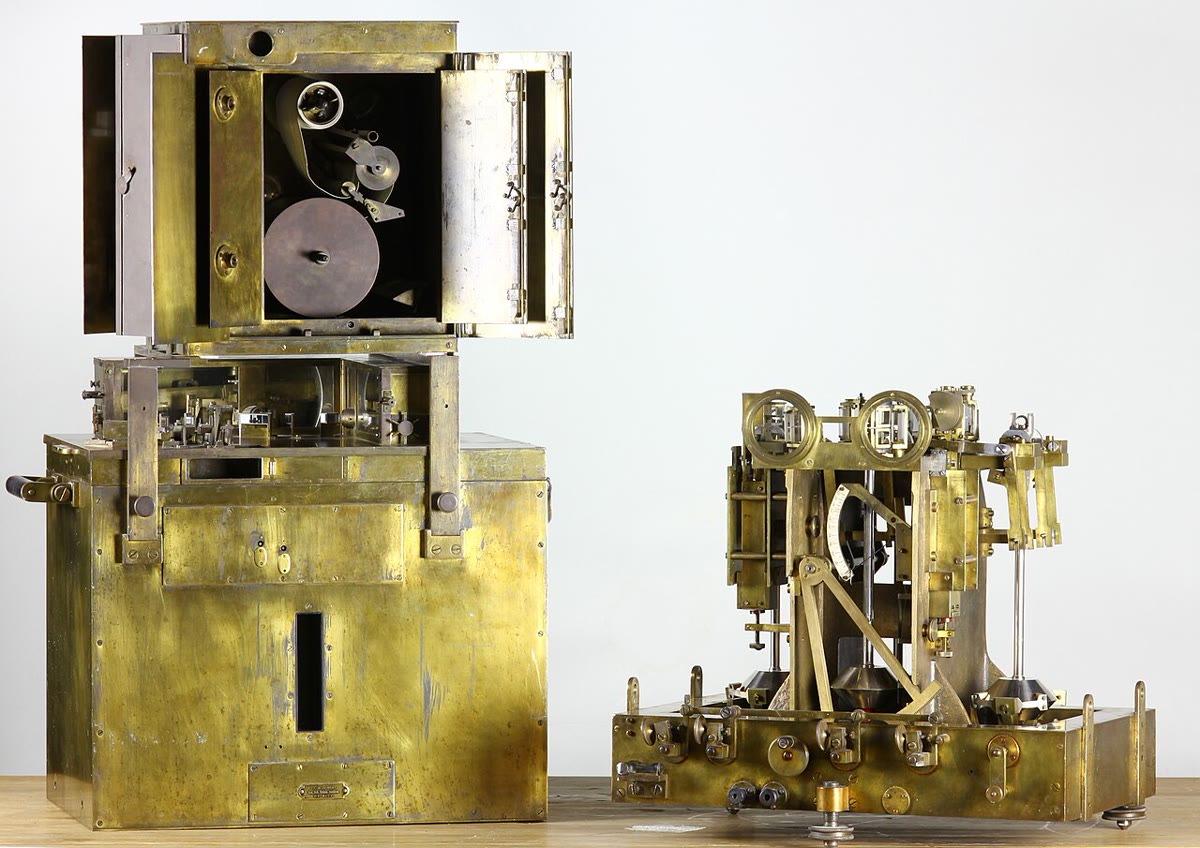
\includegraphics[width=\linewidth]{images/book3/b1-vening-meinesz.jpg}

{\scriptsize Een slingerapparaat van Vening Meinesz (rechts) en zijn kast met de registratie-eenheid
(Broodt, CC BY-SA 4.0).}
\end{minipage}
\end{history}

\section{Het geoïde}

Het zeeoppervlak in rust is een oppervlak van constante zwaartekrachtpotentiaal: als dat niet zo was, zou het water erlangs stromen. Het is het natuurlijke referentieniveau voor hoogten, en het oppervlak waar de oude schietloden loodrecht op stonden.

\begin{definition}[Geoïde; geoïdehoogte]\label{def:b1:isostasy-gravity:geoid}
Het \emph{geoïde}\index{geoïde} is het equipotentiaaloppervlak van de zwaartekracht van de aarde (gravitatie plus het centrifugale effect van de rotatie) dat samenvalt met het gemiddelde zeeoppervlak boven de open oceanen, in rust, en onder de continenten wordt voortgezet. De \emph{geoïdehoogte}\index{geoïdehoogte} $N$ in een punt is de hoogte van het geoïde boven het referentie-ellipsoïde, negatief geteld waar het geoïde eronder ligt.
\end{definition}

Hoogten boven zeeniveau op kaarten zijn hoogten boven het \omterm{def:b1:isostasy-gravity:geoid}{geoïde}; de hoogten die door satellietpositionering worden gegeven zijn hoogten boven het ellipsoïde; de twee verschillen met $N$. Het \omterm{def:b1:isostasy-gravity:geoid}{geoïde} wijkt af van het ellipsoïde met \qty{+85}{m} bij IJsland en \qty{-106}{m} voor de kust van Zuid-India, samen minder dan \qty{200}{m}, terwijl het reliëf van het vaste oppervlak ongeveer \qty{20}{km} omvat: het \omterm{def:b1:isostasy-gravity:geoid}{geoïde} is een veel gladder oppervlak dan de grond.
% ledger: nasa:geoid-range, earth:topo

\begin{proposition}[Geoïdehoogte en potentiaalanomalie]\label{prop:b1:isostasy-gravity:bruns}
Laat $\Phi$ de gravitatiepotentiaal van de aarde zijn en $\Phi_n$ de normale potentiaal, die van de modelaarde waarvan het oppervlak, het referentie-ellipsoïde, dezelfde potentiaal $\Phi_0$ heeft als het \omterm{def:b1:isostasy-gravity:geoid}{geoïde}, beide geteld met het teken van de natuurkunde (de potentiaal neemt naar boven toe, en $g = -\nabla\Phi$). Laat $T = \Phi - \Phi_n$ de potentiaalanomalie aan het \omterm{def:b1:isostasy-gravity:geoid}{geoïde} zijn. In eerste orde geldt
\[
  N = -\frac{T}{\gamma} .
\]
Geodeten, die de potentiaal met het tegengestelde teken tellen, schrijven hetzelfde resultaat als $N = T/\gamma$, de formule van Bruns.
\end{proposition}

\begin{proof}
Laat $Q$ een punt van het ellipsoïde zijn en $P$ het punt van het \omterm{def:b1:isostasy-gravity:geoid}{geoïde} op de normaal door $Q$, op de hoogte $N$. De normale potentiaal neemt naar boven toe met een snelheid $\gamma$, dus $\Phi_n(P) \approx \Phi_n(Q) + \gamma N = \Phi_0 +
\gamma N$. Omdat $P$ op het \omterm{def:b1:isostasy-gravity:geoid}{geoïde} ligt, is $\Phi(P) = \Phi_0$, dat wil zeggen
$\Phi_n(P) + T = \Phi_0$. Dus $\Phi_0 + \gamma N + T = \Phi_0$ en $N =
-T/\gamma$.
\end{proof}

Een overschot aan massa onder een punt maakt de potentiaal daar negatiever, dus $T < 0$ en $N > 0$: het \omterm{def:b1:isostasy-gravity:geoid}{geoïde} bolt op boven een overschot aan massa en zinkt bij een tekort. De \qty{85}{m} van de hoogte bij IJsland komt overeen met een potentiaalanomalie van $-\qty{85}{m}\times\qty{9.8}{m.s^{-2}} \approx \qty{-830}{J.kg^{-1}}$. Omdat de potentiaal als $1/r$ afneemt terwijl de aantrekking als $1/r^2$ afneemt, wordt het \omterm{def:b1:isostasy-gravity:geoid}{geoïde} gedomineerd door grote, diepe massa's, en de zwaartekrachtanomalieën door ondiepe. Een gecompenseerde bergketen verhoogt het \omterm{def:b1:isostasy-gravity:geoid}{geoïde} slechts weinig, omdat haar massaoverschot en het tekort van haar wortel bijna opheffen; een ongecompenseerde belasting verhoogt het veel meer.

\begin{omfigure}
\begin{tikzpicture}[x=1.15cm, y=1.3cm, font=\scriptsize, >={Stealth[length=4pt]}]
% schematic, not to scale
\fill[omSea!35] (0,0.05) .. controls (1.5,0.25) and (2.5,0.35) .. (3.6,0.45) -- (3.6,-1.2) -- (0,-1.2) -- cycle;
\fill[omLithGranite!40] (3.6,0.45) .. controls (4.5,1.4) and (5.4,1.9) .. (6.4,1.7) .. controls (7.4,1.5) and (8.2,1.2) .. (9,1.0) -- (9,-1.2) -- (3.6,-1.2) -- cycle;
\fill[omLithGabbro!35] (0,-0.7) .. controls (1.2,-0.9) and (2.4,-0.6) .. (3.6,-0.2) -- (3.6,-1.2) -- (0,-1.2) -- cycle;
\draw[thick, blue!70!black] (0,0.05) .. controls (1.5,0.25) and (2.5,0.35) .. (3.6,0.45) .. controls (5,0.75) and (7,0.75) .. (9,0.55);
\draw[thick, black, densely dashed] (0,-0.25) .. controls (3,0.05) and (6,0.15) .. (9,0.1);
\draw (3.6,0.45) .. controls (4.5,1.4) and (5.4,1.9) .. (6.4,1.7) .. controls (7.4,1.5) and (8.2,1.2) .. (9,1.0);
\node[anchor=west, blue!70!black] at (9.05,0.6) {geoïde};
\node[anchor=west] at (9.05,0.1) {ellipsoïde};
\node[anchor=west] at (9.05,1.0) {grond};
\node at (1.4,-0.3) {oceaan};
\node at (1.6,-1.0) {zeebodem};
% heights (curve ordinates computed from the Bezier segments)
\draw[<->] (6.6,0.107) -- (6.6,0.688); \node[anchor=east] at (6.57,0.40) {$N$};
\draw[<->] (7.2,0.674) -- (7.2,1.512); \node[anchor=west] at (7.23,1.09) {$H$};
\draw[<->] (8.2,0.110) -- (8.2,1.224); \node[anchor=east] at (8.17,0.95) {$h_e$};
% the vertical (perpendicular to the geoid) and the ellipsoid normal at x = 2.4 (angle exaggerated)
\draw[->, thick, blue!70!black] (2.4,0.335) -- (2.0,1.3);
\draw[->, thick, black] (2.4,0.335) -- (2.33,1.3);
\node[anchor=south east, blue!70!black] at (2.05,1.3) {verticaal (schietlood)};
\node[anchor=south west] at (2.3,1.3) {normaal op het ellipsoïde};
\end{tikzpicture}

\par\smallskip{\small Het \omterm{def:b1:isostasy-gravity:geoid}{geoïde} (blauw), het referentie-ellipsoïde (gestreept) en de grond (schematisch; afwijkingen enorm overdreven). Boven de oceaan is het \omterm{def:b1:isostasy-gravity:geoid}{geoïde} het zeeoppervlak in rust; onder het land wordt het voortgezet als equipotentiaaloppervlak. De hoogte $H$ op een kaart wordt gemeten vanaf het \omterm{def:b1:isostasy-gravity:geoid}{geoïde}, de hoogte $h_e$ die door satellietpositionering wordt gegeven vanaf het ellipsoïde, en $h_e = H + N$. Een schietlood staat loodrecht op het \omterm{def:b1:isostasy-gravity:geoid}{geoïde}, niet op het ellipsoïde: de hoek tussen beide (hier overdreven) is de afwijking van de verticaal waarmee de landmeters van India zich bezighielden.}
\label{fig:b1:isostasy-gravity:geoid}
\end{omfigure}

De afwijkingen zijn klein: de hele afwijking die de landmeters van India zorgen baarde, bedroeg ongeveer vijf boogseconden. Boven de oceanen is het \omterm{def:b1:isostasy-gravity:geoid}{geoïde} zichtbaar. Sinds 1978 meten radar-altimeters op satellieten de hoogte van het zeeoppervlak door de tijd te meten van microgolfpulsen die van het zeeoppervlak worden teruggekaatst. Als getij, golven en stromingen zijn weggemiddeld, staat het zeeoppervlak hoger boven zeebergen en ruggen en lager boven geulen en abyssale vlakten, en deze bulten (\cref{exo:b1:isostasy-gravity:11} schat er één) brengen de topografie van de diepe oceaanvloer in kaart waar geen schip heeft gepeild. De satelliet GOCE, van 2009 tot 2013, vloog op ongeveer \qty{260}{km} en mat het zwaartekrachtveld vanuit een baan, met het doel het \omterm{def:b1:isostasy-gravity:geoid}{geoïde} tot 1 tot \qty{2}{cm} en de zwaartekrachtanomalieën tot ongeveer \qty{1}{\milli\gal} te bepalen, met een resolutie beter dan \qty{100}{km}.
% ledger: pratt:himalaya, jpl:seasat, esa:goce

\subsection*{Isostasie in beweging}

\omterm{def:b1:isostasy-gravity:isostasy}{Isostasie} wordt bereikt door stroming, en stroming kost tijd. Op het hoogtepunt van de laatste ijstijd, ongeveer \num{20000} jaar geleden, bedekte een ijskap van ongeveer \qty{3}{km} dik Scandinavië. IJs is ongeveer negen tiende zo dicht als water, dus bij een \omterm{def:b1:layered-earth:layers}{mantel} van \qty{3300}{kg.m^{-3}} is de volledige isostatische indeuking onder zo'n ijskap $\qty{3000}{m}\times900/3300 \approx \qty{820}{m}$. Het ijs is verdwenen, en het land stijgt nog steeds: satellietpositionering meet vandaag tot ongeveer \qty{10}{mm.yr^{-1}} opheffing in het noorden van Zweden, ten westen van de Botnische Golf. De snelheid waarmee een indeuking zich herstelt, meet de viscositeit van de \omterm{def:b1:layered-earth:layers}{mantel} eronder, het onderwerp van Boek 5; \cref{exo:b1:isostasy-gravity:12} laat zien hoe.
% ledger: kierulf:fennoscandia, usgs:ice-density

\section{Oefeningen}

\begin{exercise}[$\star$]\label{exo:b1:isostasy-gravity:1}
(a) Reken een \omterm{def:b1:isostasy-gravity:anomalies}{Bouguer-anomalie} van \qty{-150}{\milli\gal} om in \unit{m.s^{-2}}, en druk haar uit als een breuk van $g = \qty{9.81}{m.s^{-2}}$. (b) Hetzelfde voor \qty{1}{\milli\gal}, de precisie die GOCE voor de zwaartekrachtanomalieën beoogde, en voor \qty{1}{\micro\gal}.
% ledger: esa:goce, nist:gal
\end{exercise}

\begin{exercise}[$\star$]\label{exo:b1:isostasy-gravity:2}
(a) Bereken de \omterm{def:b1:isostasy-gravity:normal-gravity}{normale zwaartekracht} aan de evenaar, op \ang{45} en aan de polen met de formule van het hoofdstuk. (b) Geef het verschil tussen evenaar en pool in milligal. (c) De centrifugale versnelling aan de evenaar is \qty{3392}{\milli\gal}. Welk deel van het verschil verklaart de rotatie rechtstreeks?
% ledger: moritz:grs80
\end{exercise}

\begin{exercise}[$\star$]\label{exo:b1:isostasy-gravity:3}
Een plateau staat \qty{3}{km} boven zeeniveau. Met een \omterm{def:b1:layered-earth:layers}{korst} van dichtheid \qty{2800}{kg.m^{-3}} en een \omterm{def:b1:layered-earth:layers}{mantel} van \qty{3300}{kg.m^{-3}}, bereken de Airy-wortel en de verdikking van zijn \omterm{def:b1:layered-earth:layers}{korst}.
\end{exercise}

\begin{exercise}[$\star$]\label{exo:b1:isostasy-gravity:4}
(a) Met hoeveel moet een zwaartekrachtmeter worden opgetild opdat zijn aflezing met \qty{1}{\milli\gal} daalt? Gebruik \qty{0.3086}{\milli\gal.m^{-1}}. (b) Een meetcampagne beoogt anomalieën tot \qty{0.01}{\milli\gal}. Tot welke nauwkeurigheid moeten de hoogten van de stations bekend zijn?
\end{exercise}

\begin{exercise}[$\star\star$]\label{exo:b1:isostasy-gravity:5}
In het model van Pratt met $D = \qty{100}{km}$ en $\rho_0 = \qty{2700}{kg.m^{-3}}$,
(a) bereken de dichtheid van de kolommen die \qty{1}, \qty{3} en \qty{5}{km} hoog staan;
(b) bereken de dichtheid van een kolom onder \qty{4}{km} zeewater met dichtheid \qty{1030}{kg.m^{-3}}. (c) Waarom past het model van Pratt beter bij de oceaanbodem dan bij de continenten?
\end{exercise}

\begin{exercise}[$\star\star$]\label{exo:b1:isostasy-gravity:6}
Twee stations liggen op \omterm{def:b1:spherical-astronomy:geographic}{breedtegraad} \ang{48}, waar de \omterm{def:b1:isostasy-gravity:normal-gravity}{normale zwaartekracht} \qty{9.808911}{m.s^{-2}} is. Station 1, \qty{350}{m} boven zeeniveau, leest \qty{9.807751}{m.s^{-2}}; station 2, op \qty{1850}{m}, leest \qty{9.803552}{m.s^{-2}}. (a) Bereken de \omterm{def:b1:isostasy-gravity:anomalies}{vrije-luchtanomalie} en de \omterm{def:b1:isostasy-gravity:anomalies}{Bouguer-anomalie} van beide, met de standaard Bouguer-dichtheid. (b) Wat suggereren de anomalieën van station 2 over de bergen eromheen?
\end{exercise}

\begin{exercise}[$\star\star$]\label{exo:b1:isostasy-gravity:7}
(a) Volg het bewijs van \cref{prop:b1:isostasy-gravity:slab} en toon aan dat een horizontale schijf met straal $a$, dikte $h$ en dichtheid $\rho$ een punt op haar as aantrekt, op een afstand $z \gg h$ erboven, met $2\pi G\rho h\,\bigl(1 -
z/\sqrt{z^2 + a^2}\bigr)$. (b) Welke straal geeft \qty{90}{\percent} van de plaatwaarde bij $z = \qty{1}{km}$? (c) Wat zegt dit over de oppervlakte van het terrein die voor de \omterm{def:b1:isostasy-gravity:anomalies}{Bouguer-correctie} telt?
\end{exercise}

\begin{exercise}[$\star\star$]\label{exo:b1:isostasy-gravity:8}
In het model van Airy met een \omterm{def:b1:layered-earth:layers}{korst} van \qty{2800}{kg.m^{-3}}, \qty{35}{km} dik op zeeniveau, boven een \omterm{def:b1:layered-earth:layers}{mantel} van \qty{3300}{kg.m^{-3}}, (a) bereken de antiwortel en de korstdikte onder \qty{4}{km} zeewater van dichtheid \qty{1030}{kg.m^{-3}}. (b) De oceanische \omterm{def:b1:layered-earth:layers}{korst} is in werkelijkheid ongeveer \qty{5}{km} dik. Wat toont het verschil? % ledger: usgs:crust-thickness
\end{exercise}

\begin{exercise}[$\star\star$]\label{exo:b1:isostasy-gravity:9}
In de inleiding was de afwijking in het verschil in \omterm{def:b1:spherical-astronomy:geographic}{breedtegraad} tussen Kaliana en Kalianpur \qty{5.236}{''}, terwijl de aantrekking van de Himalaya die Pratt berekende \qty{15.885}{''} had moeten opleveren. (a) Reken beide hoeken om in radialen. (b) Een horizontale versnelling $a_h$ kantelt een schietlood over de hoek $a_h/g$. Welk verschil in horizontale aantrekking tussen de twee stations hoort bij elke hoek, in milligal, met $g = \qty{9.79}{m.s^{-2}}$? (c) Welk deel van de aantrekking van de zichtbare bergen heeft de compensatie opgeheven?
% ledger: pratt:himalaya
\end{exercise}

\begin{exercise}[$\star\star\star$]\label{exo:b1:isostasy-gravity:10}
Een zoutkoepel wordt gemodelleerd als een bol met straal \qty{2}{km}, met zijn middelpunt op \qty{4}{km} diepte en een dichtheid \qty{200}{kg.m^{-3}} lager dan de gesteenten eromheen. (a) Toon aan dat een begraven bol met afwijkende massa $M$ op diepte $z$ op de horizontale afstand $x$ de anomalie $GMz/(x^2 + z^2)^{3/2}$ geeft. (b) Bereken de anomalie boven haar middelpunt. (c) Op welke afstand is zij gedaald tot de helft van haar piekwaarde? (d) Hoe zou de diepte van een bol uit een gemeten profiel kunnen worden afgelezen?
\end{exercise}

\begin{exercise}[$\star\star\star$]\label{exo:b1:isostasy-gravity:11}
Een zeeberg is een kegel van \qty{3}{km} hoog met een basis van straal \qty{15}{km}, die op een zeebodem van \qty{5}{km} diep staat. Zijn gesteente heeft een dichtheid van \qty{2800}{kg.m^{-3}}, zeewater \qty{1030}{kg.m^{-3}}. (a) Bereken zijn overschot aan massa boven het water dat hij verplaatst. (b) Behandel hem als een puntmassa in zijn zwaartepunt, een kwart van zijn hoogte boven de basis, en gebruik \cref{prop:b1:isostasy-gravity:bruns} met $\gamma = \qty{9.81}{m.s^{-2}}$ om de hoogte van de bult van het zeeoppervlak erboven te schatten. (c) Overschat of onderschat de puntmassa de bult? (d) Als de zeeberg volledig door een wortel was gecompenseerd, hoe zou de bult veranderen?
\end{exercise}

\begin{exercise}[$\star\star\star$]\label{exo:b1:isostasy-gravity:12}
Modelleer het herstel van Scandinavië na het ijs: stel dat het ijs \num{10000} jaar geleden plotseling verdween en een indeuking van \qty{818}{m} achterliet die sindsdien is afgenomen als $w(t) = w_0\,e^{-t/\tau}$. (a) Toon aan dat de opheffingssnelheid $w/\tau$ is. (b) Met $\tau = \num{4000}$ jaar, bereken de resterende indeuking en de opheffingssnelheid vandaag, en vergelijk de snelheid met de gemeten \qty{10}{mm.yr^{-1}}. (c) Toon aan dat $\tau = \num{3100}$ jaar en $\tau = \num{68000}$ jaar beide vandaag ongeveer \qty{10}{mm.yr^{-1}} geven. Welke resterende indeuking impliceert elk, en hoe zou een zwaartekrachtmeting tussen beide kunnen beslissen? (d) Welke eigenschap van de \omterm{def:b1:layered-earth:layers}{mantel} meet $\tau$?
% ledger: kierulf:fennoscandia
\end{exercise}

\section{Probleem: De wortel van een bergketen}

\begin{problem}[{Weekendprobleem --- de wortel van een plateau, Airy tegenover Pratt,
de zwaartekracht erboven, en wat erosie ermee doet}]
\label{pb:b1:isostasy-gravity:1}
% values: calc/ch11.py (invented plateau; normal gravity formula of the chapter)
% ledger: moritz:grs80, usgs73:reduction
Een breed plateau, enkele honderden kilometer breed, staat \qty{4}{km} boven een laagland op zeeniveau waarvan de \omterm{def:b1:layered-earth:layers}{korst} \qty{35}{km} dik is. Neem $\rho_c = \qty{2700}{kg.m^{-3}}$ voor de \omterm{def:b1:layered-earth:layers}{korst}, $\rho_m = \qty{3300}{kg.m^{-3}}$
voor de \omterm{def:b1:layered-earth:layers}{mantel}, $g = \qty{9.81}{m.s^{-2}}$, en
$2\pi G = \qty{0.0419}{\milli\gal}$ per meter per \qty{1000}{kg.m^{-3}}.

\medskip
\noindent\textbf{Deel I --- Het plateau van Airy.}
\begin{enumerate}
  \item Bereken de Airy-wortel van het plateau.
  \item Leid de dikte van zijn \omterm{def:b1:layered-earth:layers}{korst} en de diepte van zijn \omterm{def:b1:layered-earth:discontinuity}{Moho} onder zeeniveau af.
  \item Neem de \omterm{def:b1:isostasy-gravity:isostasy}{compensatiediepte} op \qty{60}{km} onder zeeniveau. Bereken de massa per vierkante meter erboven in de kolom van het plateau en in de kolom van het laagland.
  \item Bereken de druk op \qty{60}{km} diepte.
  \item Waarom is de wortel 4.5 keer de hoogte? Wat zou de verhouding zijn met een \omterm{def:b1:layered-earth:layers}{korst} van \qty{2900}{kg.m^{-3}}?
  \item Wat zou een seismische refractiemeting over de rand van het plateau laten zien als het model van Airy geldt?
\end{enumerate}

\noindent\textbf{Deel II --- Het plateau van Pratt.}
Neem nu in plaats daarvan een \omterm{def:b1:isostasy-gravity:isostasy}{compensatiediepte} $D = \qty{100}{km}$ onder zeeniveau en een kolom van het laagland met uniforme dichtheid \qty{2700}{kg.m^{-3}}.
\begin{enumerate}[resume]
  \item Bereken de dichtheid van de kolom van het plateau.
  \item Controleer dat de twee kolommen dezelfde massa per vierkante meter boven $D$ hebben.
  \item Met hoeveel procent moet de kolom van het plateau lichter zijn?
  \item Als dit dichtheidsverschil alleen door warmte zou ontstaan, met een coëfficiënt van thermische uitzetting van \qty{3e-5}{K^{-1}}, hoeveel warmer zou de kolom van het plateau dan gemiddeld moeten zijn? Is dat aannemelijk?
  \item Waar ligt de \omterm{def:b1:layered-earth:discontinuity}{Moho} onder het plateau in het model van Pratt?
  \item Een refractiemeting vindt de \omterm{def:b1:layered-earth:discontinuity}{Moho} op \qty{52}{km} onder het plateau. Welk model past?
\end{enumerate}

\noindent\textbf{Deel III --- Zwaartekracht boven het midden.}
\begin{enumerate}[resume]
  \item Bereken de \omterm{def:b1:isostasy-gravity:anomalies}{Bouguer-correctie} voor een station op het plateau.
  \item Voorspel de \omterm{def:b1:isostasy-gravity:anomalies}{vrije-luchtanomalie} en de \omterm{def:b1:isostasy-gravity:anomalies}{Bouguer-anomalie} in het midden als het plateau niet gecompenseerd zou zijn.
  \item Voorspel ze voor het plateau van Airy, en controleer de \omterm{def:b1:isostasy-gravity:anomalies}{Bouguer-anomalie} met de ontbrekende massa van de wortel.
  \item Een station in het midden van het plateau, op \omterm{def:b1:spherical-astronomy:geographic}{breedtegraad} \ang{30} en \qty{4000}{m}, leest \qty{9.781085}{m.s^{-2}}. Bereken de \omterm{def:b1:isostasy-gravity:normal-gravity}{normale zwaartekracht} op \ang{30}, en daarna de \omterm{def:b1:isostasy-gravity:anomalies}{vrije-luchtanomalie} en de \omterm{def:b1:isostasy-gravity:anomalies}{Bouguer-anomalie}.
  \item Welk deel van het plateau is gecompenseerd?
  \item Zou de \omterm{def:b1:isostasy-gravity:anomalies}{Bouguer-anomalie} in het midden anders zijn als het plateau op de manier van Pratt was gecompenseerd? Verklaar.
  \item Schets de \omterm{def:b1:isostasy-gravity:anomalies}{vrije-luchtanomalie} langs een profiel over één rand van het plateau, en verklaar de vorm ervan.
\end{enumerate}

\noindent\textbf{Deel IV --- Erosie.}
Rivieren verwijderen een laag van \qty{1}{km} dik van het hele oppervlak van het plateau, langzaam genoeg opdat de \omterm{def:b1:isostasy-gravity:isostasy}{isostasie} kan bijblijven.
\begin{enumerate}[resume]
  \item Wat is de nieuwe dikte van de \omterm{def:b1:layered-earth:layers}{korst}, en de nieuwe Airy-wortel?
  \item Wat is de nieuwe hoogte van het plateau?
  \item Met hoeveel is het gesteente dat nu aan het oppervlak ligt omhooggekomen?
  \item Hoeveel gesteente moet in totaal worden geërodeerd om het plateau tot zeeniveau te laten zakken? Wat zegt dat over de gesteenten die in oude bergketens worden gezien?
  \item Met hoeveel daalt het oppervlak van het plateau voor elke kilometer gesteente die wordt geërodeerd?
\end{enumerate}
\end{problem}
